\documentclass[letterpaper,12pt]{article}
\usepackage{graphicx,amsmath} % support the \includegraphics command and options
\usepackage{color}
\usepackage{hyperref,float}
\usepackage{dgjournal} 
%\usepackage{mathptmx}
\usepackage[authoryear,comma,longnamesfirst,sectionbib]{natbib} 


\newcommand{\blind}{0}
\newcommand{\andyc}[1]{[{\color{red}\sc Andy comment: {\tt #1}}]}

\newenvironment{blockquote}{%
  \par%
  \medskip
  \leftskip=4em\rightskip=2em%
  \noindent\ignorespaces}{%
  \par\medskip}

\oddsidemargin=0.25in
\evensidemargin=0.25in
\textwidth=6in
\textheight=8.75in
\topmargin=-.5in
\footskip=0.5in

\graphicspath{{figures/}{../figures/}}

\begin{document}

\if0\blind
{
\title{Nearest-Neighbor Matchup Effects:  Accounting for Team Matchups for Predicting March Madness}
 \author{Andrew Hoegh, Marcos Carzolio, Ian Crandell, Xinran Hu, Lucas Roberts, \\Yuhyun Song, and Scotland Leman\\
 Department of Statistics, Virginia Tech}        
  \originalmaketitle
  \begin{abstract} 
\noindent
Recently, the surge of predictive analytics competitions has improved sports predictions by fostering data-driven inference and steering clear of human bias. This article details methods developed for Kaggle's \emph{March Machine Learning Mania} competition for the 2014 NCAA tournament. A submission to the competition consists of outcome probabilities for each potential matchup. Most predictive models are based entirely on measures of overall team strength, resulting in the unintended ``transitive property.'' These models are therefore unable to capture specific matchup tendencies. We introduce our novel nearest-neighbor matchup effects framework, which presents a flexible way to account for team characteristics above and beyond team strength that may influence game outcomes. In particular we develop a general framework that couples a model predicting a point spread with a clustering procedure that borrows strength from games similar to a current matchup. This results in a model capable of issuing predictions controlling for team strength and that capture specific matchup characteristics.
\end{abstract}

\noindent%
{\it Keywords:}  Matchup effects, transitivity, relative strength, $K$ nearest neighbors
} \fi

\if1\blind
{
} \fi

\newpage
%% Do NOT include any fronmatter information; including the title, author names,
%% institutes, acknowledgments and title footnotes (author information, funding
%% sources, etc.). Start the document with the first section or paragraph of
%% the article.



%%%%%%%%%%%%%%%%%%%%%%%%%%%%%%%%%%%%%%%%%%%
%%%%%%%%%%%%%%%%%%%%%%%%%%%%%%%%%%%%%%%%%%%

\section{Introduction}
Since the advent of the NCAA basketball tournament -- informally known as \emph{March Madness} -- millions of people have taken to predicting the outcome of the tournament. There are numerous ways one might go about making such predictions. Typical strategies include using tournament seeds, listening to expert opinion from commentators or analysts, following one's intuition or biases, or using a more data-driven analytical approach. 

The rise in popularity of sports analysts such as Nate Silver from FiveThirtyEight \citep{silver} and Bill James from \emph{Moneyball} \citep{james, moneyball} has dramatically increased the visibility of data-driven methods for sports predictions. This trend has culminated in a growing number of amateur analysts having their hand at sports predictions. 

Prediction challenges, such as the one hosted by Kaggle in 2014 \citep{kaggle}, have sprung onto the scene to provide a venue for comparing such analysts' results. 
In contrast to a typical bracket competition, Kaggle's requires competitors to compute winning probabilities for every potential tournament matchup (2,278 in total). This article stems from our team's submission to this competition and contains an explanation of our modeling framework specifically designed to capture matchup effects. 
%%%%%%%%%%%%%%%%%%%%%%%%%%%%%%%%%%%%%%%%%%%
\subsection{March Madness Prediction \label{methods_review}}
In recent years, an abundance of research has accumulated aimed at predicting sporting outcomes. \cite{boulier2003predicting} provide a comprehensive review, showing that measures of strength based on  rankings/seeds, power scores as calculated by The New York Times,  and Las Vegas bookmakers are useful for accurately predicting such games. \cite{smith1999can} showed previously that tournament seeds and resulting point spreads have a linear relationship, rendering them useful as simple baseline game predictors. Jeff Sagarin \citep{sagarin} provides a more sophisticated methodology for calibrating point spreads, based on team winning percentages and historical records of game point differentials. 

Constant refinements have been made to improve the accuracy of such predictions. While correctly predicting point spread is useful when determining a game's outcome, the spreads exhibit increasing variability as actual team scores increase. To compensate, 
\cite{caudill2003predicting} evokes a nonparametric method for estimating maximum scores -- a method originally developed by \cite{manski1977estimation}.
Applying this technique to March Madness from 1985 to 1998, the author showed that the method improved upon traditional parametric models. While such nonparametric methods have shown promise, enhanced parametric models remain the mainstay of sports prediction. For instance, a recent study based on ordinal logistic regression \citep{west2006simple} created an ordinal ranking scheme for gauging teams on a scale of 0 to 6. 

Along these parametric lines, many have invoked simple linear frameworks utilizing a multitude of features for game prediction. For instance, \cite{wright2012statistical} modeled both winning margins and binary game results using linear regression and probit regression, respectively. The key feature was to include a multitude of covariates as predictors: tournament seeds, winning percentages in the regular season, Sagarin rankings, and points per game. Expanding on this, \cite{rosenthal} considered multiple constrained regression models and applied a Monte Carlo search algorithm for predicting game outcomes. While the overall structure slightly extends upon simple linear approaches, one of Rosenthal's key contributions was the data used in the model: regular season win percentage, final three game win percentages, offensive and defensive efficiency ratings, strength of schedule, and out-of-conference win rates. These measures go well beyond simple team strength metrics. A similar method, which has gotten a lot of attention in recent years due to its accuracy is the Logistic Regression / Markov Chain (LRMC) method by \cite{Kvam2006}. While this method does not consistently outperform others in the regular season, it has shown a high degree of accuracy in the NCAA tournament.
%%%%%%%%%%%%%%%%%%%%%%%%%%%%%%%%%%%%%%%%%%%
\subsection{Transitivity and Matchup Effects}
On Thursday, May 20, 2014, before the start of the 2014 NCAA tournament, Andy Enfield -- head coach of USC Men's Basketball, and former head coach of the 2013 Florida Gulf Coast team that had the deepest run in the history of the NCAA tournament by a 15 seed -- made an appearance on the ESPN radio program First Take. When asked about potential upsets, he responded as follows. 
% Listen here: https://www.youtube.com/watch?v=pAERNPdUiC8#t=1966
\begin{blockquote}
\indent Well, it's hard to predict a particular team. You have to look at the higher seed and see, do they overwhelm the smaller school or the lower seed? Can they overwhelm someone with their athleticism or length or size or quickness or speed? Do they play a particular style of the pressure defense? And I think I look at the lower seed then and say, can they counter the higher seed's strengths? Do they shoot the three point shot well? Do they have athleticism at certain positions? Do they play a particular style that will give the higher seed trouble? 
\indent And as I look at the tournament I see a team like Delaware with three great guards that average 57 points a game between them. You look at a team like Michigan State that can overwhelm a team with their athleticism and size. So I think that'll be an interesting first round matchup. You look at a team like Mercer who has a great point guard in Langston Hall and a 6'11" center who's an all-league player versus Duke's overwhelming athleticism and size on the wing, so there's some very interesting matchups, and I look forward to it.
\end{blockquote}
\noindent Michigan State went on to overwhelm Delaware with a 93-78 win. No. 14 seed Mercer upset No. 3 seed Duke 78-71. Mercer shut down Duke's post game and in exchange granted them the ability to take outside shots, which Duke missed almost all game long.

Coach Enfield's implication is that a team's performance depends on the kind of team it is playing -- what we dub the matchup effect. More formally, a matchup effect is any term in a predictive model that depends on the interaction between both teams. 

Unfortunately many of the methods detailed in Section 1.1 are based on overall team strength and are therefure unable to handle specific matchups. These methods impose a relation known as the transitive property. This notion of transitivity states that if team A is expected to beat team B and team B is expected to beat team C, then team A is also expected to beat team C. Formally, if $P_{A>B}$ denotes the probability that team $A$ beats team $B$, then for any teams A, B, and C: 
\begin{eqnarray*}
\left \{P_{A>B} > 0.5 \quad \cap \quad P_{B>C} > 0.5 \right\} \implies P_{A>C} > 0.5.
\label{eq:trans}
\end{eqnarray*}

The key point is that models with this property strictly rely on estimates of team strength and do not account for specific tendencies of a given matchup. Clearly models of this type are unable to handle matchup-specific tendencies. To accommodate this, we develop the Nearest-Neighbor Matchup Effects (NNME), which provide a flexible method to capture specific tendencies of teams and make predictions that are not restricted to transitivity. This framework, in spirit, can be applied to any modeling approach and will allow for non-transitive relationships between games.

The remainder of the article is as follows: Section 2 discusses relevant data, Section 3 outlines the Nearest-Neighbor Matchup Effects, Section 4 demonstrates the efficacy of the modeling framework with matchup effects, and Section 5 concludes with a discussion.
%%%%%%%%%%%%%%%%%%%%%%%%%%%%%%%%%%%%%%%%%%%
%%%%%%%%%%%%%%%%%%%%%%%%%%%%%%%%%%%%%%%%%%%
\section{Data}
The key ingredient for any analytic approach to prediction is quality data. While many influential factors exist for predicting college basketball games, a common approach uses game-level data that has been aggregated to reflect team characteristics. These characteristics include winning percentage, average point differential, and home court advantage, which is consistently shown to be worth about 4 points on average \citep{harville1994}. The goal with this type of model is to construct a latent measure of team strength with which teams can be compared. 

An alternative approach to computing team strength from a set of team characteristics is to use one or more of the preexisting rating systems. With the large number of people working in this area -- Ken Massey \citep{kenmassey.com} providing nearly 70 different systems -- it is no surprise that the best of these rankings work quite well. For instance, basing predictions on such rankings alone, we find that 70-75\% of all game outcomes could be correctly classified. While incorporating more factors only improves this figure by a few percent, these factors can be useful in correctly calibrating the point differentials for each game. The point differentials, in turn, become greatly influential in subsequently calibrating the outcome probabilities for each game.

While some of the algorithms are proprietary, we provide a brief overview of the main ranking systems. Currently, the NCAA selection committee selects 36 teams (at large bids) in addition to 32 conference champions (automatic bids) and places these 68 teams into competing brackets. The seeding system, which rates teams 1 through 16 within each region is well known. A lesser known rating is the so called `S-curve' which gives an ordinal ranking of each team in the field. This ranking is decided on by a 10 person committee, and is not generated by a systematic, model-based approach. 

On the other hand, the LRMC method \citep{Kvam2006, mark2010} is a two-step procedure used to produce ordinal rankings of each team. The first step evaluates every game played during the season to compute the probability that one team is better than the other team. This step uses the score at the end of regulation (\emph{i.e.} overtime results are not included) and the home team in a logistic regression setting. The second step uses these probabilities in a Markov chain to produce the ordinal rankings. Specifically, each team is given a state in the chain based on the head-to-head probabilities and the ordinal ranking is a result of the ordering for the steady state probabilities of the chain.

Among the top performing off-the-shelf models is Jeff Sagarin's computer ranking system, known simply as the Sagarin rankings \citep{sagarin}. Sagarin rankings are a staple because of both their longevity -- they have been used since 1985 -- and their quality. The exact methodology is unknown, but the Sagarin rating is actually a composition of three separate models. One model uses only wins or losses without regard to point differential, while the other two focus primarily on point spreads. A characteristic of the Sagarin rankings is that the difference in team ratings represents the expected point spread for that matchup on a neutral court, making this a natural baseline metric for predicting point speads. For the 2013-2014 year, Sagarin estimated the home court advantage at 3.38 points.

The Pomeroy rankings, developed by Ken Pomeroy \citep{kenpom.com}, are largely driven by the Pythagorean expectation, which was originally used by Bill James for baseball prediction \citep{james}, and follows as:
\begin{eqnarray}
E[Pr(Win)] = \frac{pt_s^c}{pt_s^c + pt_a^c},
\end{eqnarray}
where $pt_s$ and $pt_a$ denote seasonal points scored and allowed, respectively, and $c$ is a tunable constant, which Pomeroy estimates at $10.25$.  
A theoretical derivation of the Pythagorean expectation is provided by \cite{miller2007}.
Rather than actual points scored, Pomeroy uses adjusted and defensive efficiencies as inputs into the Pythogorean expectation.

Table \ref{tab:ranks} contains pre-tournament ordinal rankings for the top 16 seeds in the NCAA tournament as well as the eventual national champion Connecticut, from the Sagarin, Pomeroy, LRMC models as well as the S-curve itself.

\begin{table}[h!]
\caption{Pre-tournament Ranking Comparison}
\footnotesize
\centering
\begin{tabular}{l|ccccc|c}
  \hline
  \hline
 Team & Sagarin Rank &  Pomeroy Rank  & LRMC Rank & S-Curve& Ave. Rank  \\ 
  \hline
 Arizona         & 1  &1      & 2 & 2& 1.5  \\
 Florida          & 3  &3      &3 & 1& 2.5\\
 Louisville      & 2  &2      & 1 &13 & 4.5\\
 Virginia         & 5  &4       &8 & 4 &5.25\\
  Kansas         & 6  &8      & 4& 7 &6.25\\
 Villanova      & 4  &7       & 9 & 5 &6.25\\
 Wichita St    & 12 &5          &5 & 3 &6.25\\
 Duke             & 7  &6         &6 &9&7\\
  Creighton &  11 &   9   &7 &11& 9.5\\ 
 Wisconsin  &   9   &13     &  11 & 8 &10.25\\
 Michigan St & 8  &10   & 12& 14&11\\
 Michigan & 10 & 15&  16& 6 &11.75\\
 UCLA & 15& 18& 10 &15 &14.5\\
 Iowa St &13 &23  &19 &12 &16.75 \\
 Syracuse &19 &14   &24 &10 &16.75 \\
 San Diego St&22 &21   &25 &16 &21 \\
  \hline
  Connecticut & 24& 26& 26& 26&25.5\\
  \hline
   \hline
\end{tabular}
\label{tab:ranks}
\end{table}

These seeds and rankings contain implicit or explicit means for tournament prediction. For instance the Sagarin ratings are designed to reflect the point spread between two teams, incorporating a term for the variance of the outcomes under a Bayesian framework provides an efficient way to compute win probabilities. Similarly any of the other rankings can be used for predicting point spreads or in a binary regression framework. For instance, a seed-based probability is shown in \cite{schwertman1996}, while a more sophisticated approach using point spreads along with Sagarin's rankings is demonstrated in \cite{carlin1996}. There are some similarities, but each of the ranking system has its own flavor as seen in Table \ref{tab:ranks}. Saying that, each is useful in gauging a team's strength, and the collection helps quantify the uncertainty in such measurements.

\subsection{Data Treatment}
A necessary consideration when modeling game outcomes is whether the outcome of a game is binary (win/loss) or continuous (point differential). Point spread provides a means for measuring the relative strength of one team versus another. However, as any basketball fan can attest, the final score is often not indicative of the closeness of the game. This can go either way as fouling in the final minutes leads to inflated point differentials; or conversely, teams with a big lead at the half will clear the bench and put in the reserves,  usually decreasing the differential. Nevertheless, point spreads are informative about the relative strength of one team compared to another. In practice, given a distribution (posterior in our case) of point spreads, we can compute and calibrate winning probabilities. Preliminary data analysis suggests that modeling binary outcomes is inferior to modeling the point spread. 

When modeling point differentials, converting point differentials $y_{(i,j)}$ to probabilities $Pr(y_{(i,j)}>0)=p_{(i,j)}$ is a fundamental requirement. Given a Bayesian viewpoint, we compute the overlap of the posterior predictive distribution of the point spread with the positive axis. Mathematically this is expressed as $\int_0^\infty p(y_{(i,j)})dy_{(i,j)}$. See Figure \ref{fig:winprob}, for an illustration where  $p(y_{(i,j)}) \sim N(5,10^2)$ which equates to a game winning probability: $p_{(i,j)}=0.69$.
We again note that while binary outcome models offer these probabilities automatically, the point spread models are able to account for more information. 
\begin{figure}[h!]
\centering
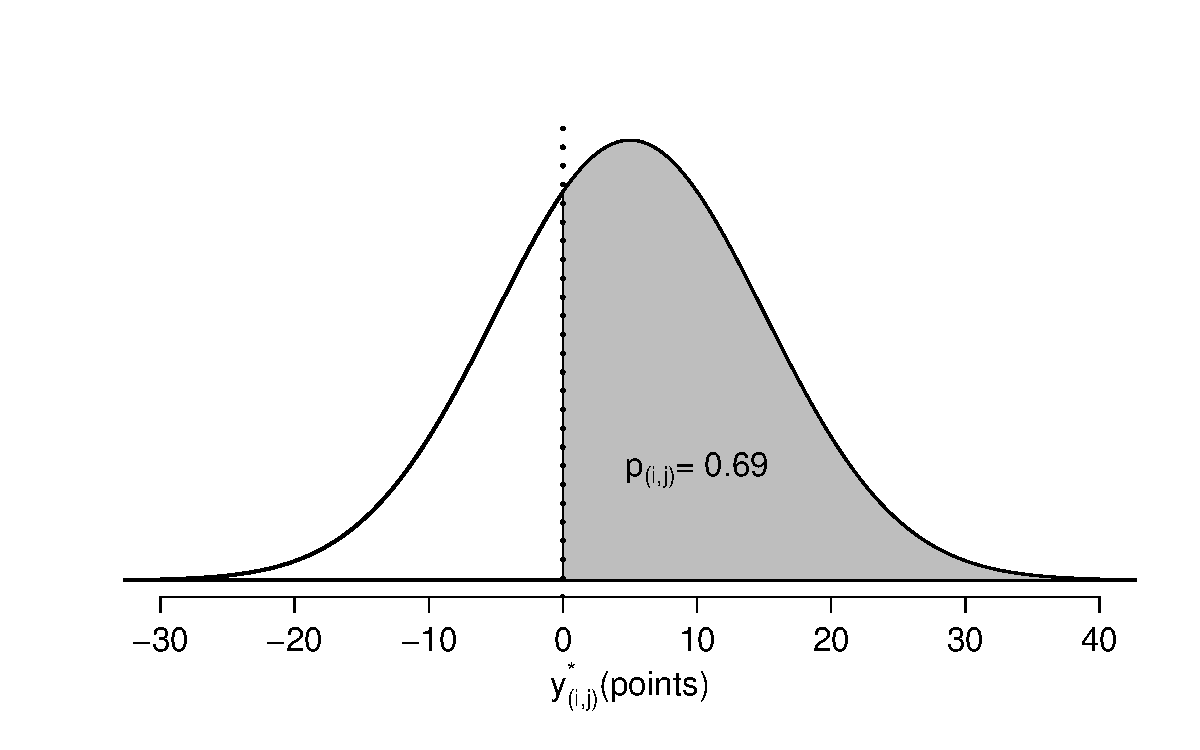
\includegraphics[width=.7\textwidth]{WinProb2.pdf}
\caption{Calculating win probability $(p_{(i,j)}),$ where $p(y_{(i,j)}) \sim N(5,10^2)$.}
\label{fig:winprob}
\end{figure} 

\section{Modeling\label{sec:NNME}}
Before describing our nearest-neighbor matchup effects framework, we first detail a general class of models called additive relative strength models. These models are a class of models for predicting point spreads of matchups. The drawback is that these models are not able to capture specific characteristics of a matchup, rather relying on estimates of overall team strength. Despite being transitive (and unable to handle matchup tendencies), the class of models will be a building block for computing matchup effects. Furthermore, this allows us to easily discuss the marginal improvements achieved via incorporating matchup effects. 

NNME is a three-step process: (i) fit an additive relative strength model, (ii) identify neighbors by finding similarities between the current opponent and past opponents for each team, and (iii) calibrate the matchup adjustment. Additive relative strength models are a relatively straightforward approach on their own; however, accounting for matchup effects through our proposed nearest-neighbors approach adds a layer of novelty and ultimately enhance our predictions. In some sense, team strength is computed and averaged across a complete set of opponents. We seek a homogenous subset of opponents similar to the current matchup to assess the performance against that group. Section \ref{sec:AS} provides a general overview of the framework, while Section \ref{sec:demon} shows our method applied to the 2014 NCAA tournament and demonstrates the effectiveness of our approach.

\subsection{Additive Relative Strength Models \label{sec:AS}}
We first detail a general class of models for predicting point spread, which includes many of the simple to sophisticated regression techniques presented in Section \ref{methods_review}. These models can be written in a general form as:
\begin{eqnarray}
Y_{(i,j)} = g_1\left(D_{(i,j)}\right) + g_2\left(X_{(i)}\right) + g_3\left(X_{(j)}\right) +  \epsilon_{(i,j)},
\label{eq:RS}
\end{eqnarray}
where $Y_{(i,j)}$ denotes the point spread (team $i$ - team $j$), and $\epsilon_{(i,j)}\sim N(0,\sigma^2)$ represents the model error. The model covariates include team specific covariates $(X_{(i)}$, $X_{(j)})$ as well as differences between team covariates ($D_{(i,j)}$). Where for example $D_{(i,j)}$ might be the difference in Sagarin ratings for team $i$ and team $j$. The functions $g_i$ represent any possible function modeling the dependency between covariates and point spread, which forms a Generalized Additive Modeling (GAM) framework \citep{GAMs}. Equation \ref{eq:RS} only accounts for additive effects. These additive effects, based on measures of team strength, are not always sufficient for capturing key characteristics of matchups. In order to account for these characteristics, we search for a subclass of opponents in which strengths or weaknesses are similar, and build a local network which shares information across like neighbors.  

While we explored various functions $g_i$ for the additive relative strength component of our model and settled on a relatively simple linear structure:
\begin{eqnarray}
Y_{(i,j)} =  \beta_{home} + D_{(i,j)}\beta_D +  \epsilon_{(i,j)},
\label{eq:RS2}
\end{eqnarray}
where $\beta_{home}$ is a term for home court advantage, $D_{(i,j)}=\{(Sagarin_{i,1} - Sagarin_{j,1})\}$ is the difference in Sagarin ratings between team $i$ and team $j$, and $\epsilon_{(i,j)} \sim N(0,\sigma^2).$ This model is fit via a Bayesian framework by placing vague conjugate priors on $\pi(\beta_{home})\propto 1, \pi(\beta_D) \propto 1,$ and $ \pi(\sigma^2) \propto \frac{1}{\sigma^2}$. While this model is relatively simple it has produced good results historically \citep{carlin1996} and provides an interpretable framework for evaluating the efficacy of incorporating matchup effects. As NCAA tournament games are played in neutral settings this model will reduce to the case where $\beta_{home}$ is excluded.

\subsection{Identifying Neighbors}
The second component of computing matchup effects consists of identifying similar opponents to the current foe. Consider a matchup between team $i$ and team $j$, we borrow strength by identifying past opponents with similar characteristics to the current foe for both teams $i$ and $j$. The idea is to identify how the performance changes against the subset of opponents which are similar to the current opponent. This subsection focuses on methods for identifying similarities between teams and selecting neighbors.

Neighbors are selected in an unsupervised framework using a large set of team-level data. In particular we use a selection of variables aggregated by Ken Pomeroy \citep{kenpom.com} for similarity calculations pertaining to: team height, tempo, scoring characteristics, rebounding,  assist rate, shooting percentage, and defensive characteristics. A complete list of variables and an overview of their meaning is provided in Appendix A. Typically this procedure is done analytically, after standardizing the variables, however, user input can also be elicited. For instance, suppose that a user decided Mercer was similar to Wake Forest and Clemson due to their size and playing style. In this case, current work under the Bayesian Visual Analytics (BaVA) paradigm \citep{house2010, hu2013} provides a principled routine for visualizing teams and taking user inputs to compute similarities between teams in a semi-supervised manner. Specifically, BaVA is a way to weight clustering variables to reflect user preferences.

For our application BaVA principles are not applied. Rather, we standardize the set of variables and calculate the Euclidean distance between team $j$ and all of team $i's$ past opponents, and vice versa. Given the computed (dis)similarities between team $j$ and team $i$'s past opponents, we select the $K$ teams most similar to team $j$. This selection of teams are the $K$-nearest neighbors for team $i$ representing past opponents most similar to the current opponent. Note we are not quite using the $K$ nearest neighbors algorithm for prediction, but rather we are using these teams to borrow strength (from similar teams) in a similar fashion.

\subsection{Matchup Adjustment}
Our matchup effects adjustments can be applied to any additive framework. The final element of the matchup effects is to apply the matchup adjustment. The idea of the matchup adjustment is to quantify how much a team over- or under-performed relative to the expected team strength for a subset of teams similar to the current opponent. For instance, if team $i$ was two points better than expected given team strength against teams similar to $j$, then it would be reasonable to assume that team $i$ would perform better than expected against team $j$ as well. Computing the matchup adjustment is a three step procedure: 1) fit a relative strength model, 2) compute the average of the residuals against the identified set of neighbors, and 3) augment the relative strength model with an additive adjustment corresponding to the performance against similar teams.

Given a distribution of predicted point spreads for a matchup between team $i$ and team $k$, let $\mu_{(i,k)} = E[y_{(i,k)}|X_{(i,k)}]$. That is $\mu_{(i,k)}$ is the expected point differential, whereas $y_{(i,k)}$ is the realized point differential between teams. Then define:
\begin{eqnarray*}
\mathcal{N}_j(i) = \frac{1}{K}\sum_{k_j=1}^K \left(y_{(i,k_j)} - \mu_{(i,k_j)}\right)
\end{eqnarray*}
where $k_j = 1,...,K$ are the identified neighbors of team $j$. The term $\mathcal{N}_j(i)$ represents the average residual for team $i$ against the set of neighbors of team $j$, which describes in essence how much a team over- or under-performs its expected performance. If $\mathcal{N}_j(i)$ is greater than zero, then team $i$ typically out performs against teams like team $j$. In other words this term can be thought of as the difference in expected performance against teams like team $j$ after accounting for team strength. Given $\mathcal{N}_j(i)$ and $\mathcal{N}_i(j)$, we define the matchup effect by:
\begin{eqnarray}
\phi_{(i,j)} &=& \rho(\mathcal{N}_i(j) -\mathcal{N}_j(i)),\label{eq:phi}
\end{eqnarray}
where $\rho \in [0,1]$ is a tuning parameter that controls the amount of information passed between neighbors. Effectively, if $\mathcal{N}_i(j) >0$ and $\mathcal{N}_j(i)<0$, then we we would deem that team $i$ will tend to perform better than expected against team $j$ and team $j$ will perform worse than expected against team $i$. Hence, $\phi_{(i,j)}$ represents a shift in the distribution of point spreads between teams $i$ and $j$. Using the model from Equation \ref{eq:RS2} and applying Equation \ref{eq:phi}, then the predictive distribution for a matchup between team $i$ and team $j$ now becomes
\begin{eqnarray}
Y_{(i,j)}|X_{(i,j)} &=& \beta_{home} +  D_{(i,j)}\beta + \phi_{(i,j)} +  \epsilon_{(i,j)k} \label{eq:ME}.
\end{eqnarray}
The same idea applies to the more general models such as Equation \ref{eq:RS}, or any other additive approach, which may enhance the predictiveness of the method. Looking at Equation \ref{eq:ME} we see the result of the matchup effect is a mean shift in the point spread, which results in an updated probability calculation.

\subsubsection{Model tuning\label{sec:tuning}}
The matchup effects, in essence, help minimize residual errors in predicting point spreads. In spirit, this analysis could be conducted jointly; however, in order to expedite some of the computations, we run the model in sequence. That is, we first fit Equation \ref{eq:RS2}, and then incorporate matchup effects. The amount of error controlled by this adjustment is calibrated by tuning $\rho$. 

The interpretation at the extreme points of $\rho$ is intuitive: setting $\rho = 0$ reverts Equation \ref{eq:ME} to Equation \ref{eq:RS2}, and setting $\rho = 1$ applies the entire value of $\mathcal{N}_i(j) -\mathcal{N}_j(i)$. To select $\rho$ in practice, we use a cross-validation procedure. Specifically we compute an optimal value of $\rho$ across seven years of historical data and use that value for predictions for this year's tournament. Similarly, the number of neighbors ($k$) in the analysis is simultaneously selected under cross-validation. We found values of $\rho$ near 0.2 to work quite well. Shrinking the matchup effect with $\rho <1$ still borrows strength in estimation from similar teams, but guards against overfitting.


\section{Demonstration \label{sec:demon}}
To demonstrate the efficacy of the NNME, we provide a comparison of the standard Sagarin model (Equation \ref{eq:RS2}) with a model using matchup effects (Equation \ref{eq:ME}). For notational purposes, we denote these models as $M_{rs}$ and $M_{me}$, respectively. Evaluation is conducted in the same manner as the Kaggle competition, where participants are required to enumerate game winning probabilities (probability of team A beating team B, for all $68 \choose 2$ pairs). Based on these predicted game wining probabilities, the following loss function is used:
\begin{equation}\label{eq:kaggle_score}
L(y,p)=-\sum_{i=1}^n\frac{y_ilog(p_i)+ (1-y_i)log(1-p_i)}{n},
\end{equation}
where $p_i\in[0,1]$ is the probability team $i$ wins and $y_i=1$ if team $i$ wins and $y_i = 0$ if team $i$ loses.

Data is obtained that includes regular season and NCAA tournament games from the present year (2014) as well as the preceding seven years. All regular season games featuring Division 1 teams are used to fit a relative strength model for each year with the Sagarin rankings as predictors as shown in Equation \ref{eq:ME}. Given the conjugate priors specified in Section \ref{sec:AS}, the relative strength model is fit using a Gibbs sampler. Then NCAA tournament games are used to calibrate the tuning parameter $\rho$. For any given year, the optimum will vary, ranging from 0 to 0.70. However, for predictions we select the value of $\rho$ that minimizes the loss across the seven preceding years of data that are used for calibration. This value is stable around 0.2.

 \subsection{Results}
Applying the $M_{me}$ model results in an improvement over the $M_{rs}$. Table \ref{tab:results} shows the final loss and overall ranking in the Kaggle competition for each method (to provide context for the differential in the loss between the two methods).

\begin{table}[h!]
\caption{Overall loss and Kaggle Ranking for comparison models.\label{tab:results}}
\centering
\begin{tabular}{|c|cc|}
  \hline
    & Loss & Ranking\\ 
  \hline
  $M_{RS}$ & .58497 & 97 \\
  $M_{ME}$ & .57909 & 85 \\
   \hline
   \hline
\end{tabular}
\end{table}

Furthermore, Figure \ref{fig:result} shows how the Kaggle loss function varies as a function of $\rho$. The dashed line shows the optimal value of $\rho$ across 7 years of historical data ($\approx .2$); whereas, the solid line shows the optimal value of $\rho$ for the 2014 season ($\approx 0.35$). 
\begin{figure}[h!]
\centering
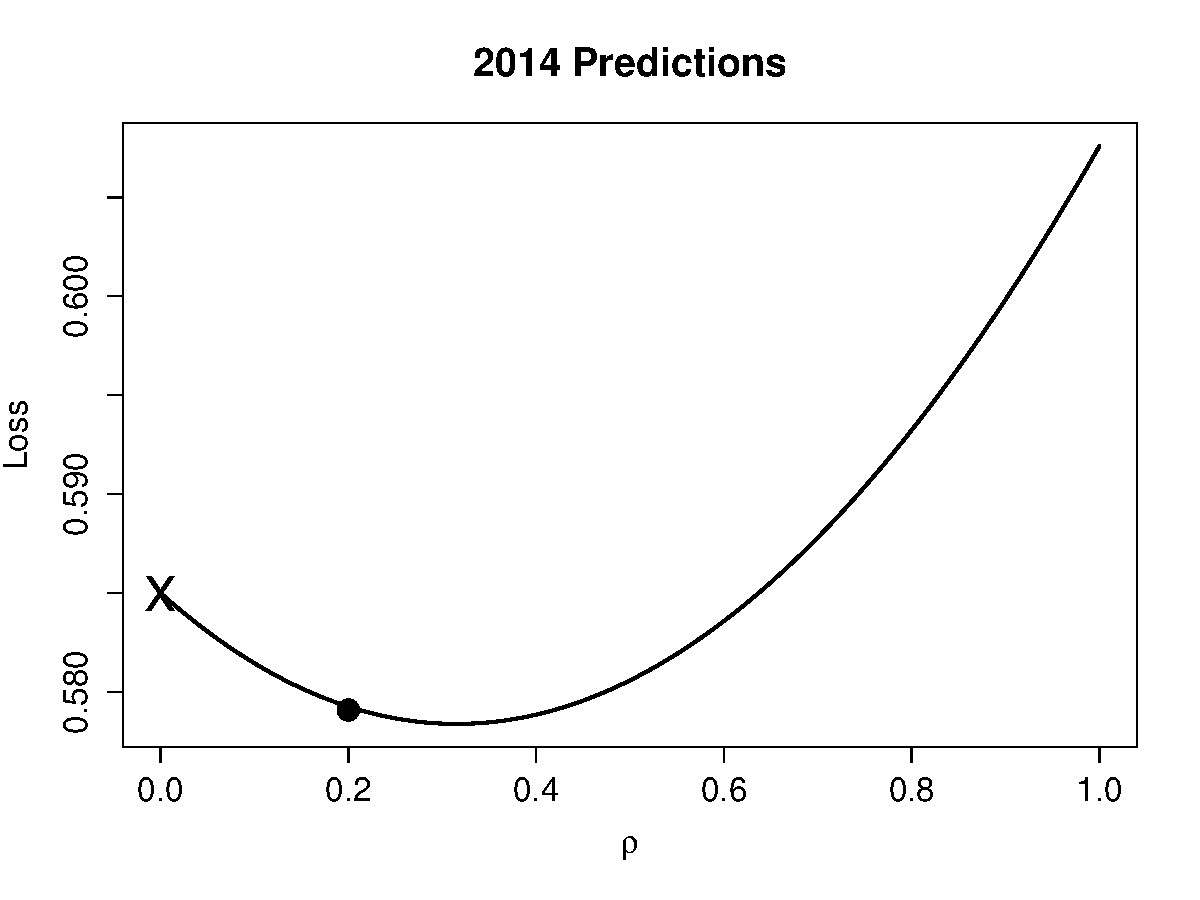
\includegraphics[width=.8\textwidth]{Predictions.pdf}
\caption{Kaggle loss as a function of $\rho$ for 2014 NCAA tournament. The {\bf X} denotes $M_{RS}$ where $\rho = 0$ and the black dot denotes $M_{ME}$ with $\rho$ selected based on 7 years of historical data.}
\label{fig:result}
\end{figure} 

It is important to note that implementing NNME will not drastically alter the results from a relative strength model. In fact most of the predictions between the two models will be extremely similar. This occurs when neither opponent sets up as a particularly favorable or unfavorable matchup. However, for cases where an advantage or disadvantage is identified we can see the expected point spread shift up to three or four points. Collectively, shifting the point spread, and in turn adjusting calibrated probabilities for a select group of games can result in a meaningful difference in predictions. 

We further explore the enhancement that our matchup effects model improves over the relative strength model by examining games with the largest matchup effects. Table \ref{tab:change} shows the ten games which saw the largest shift in expected point spread. Table \ref{tab:change} displays these expected point spreads ($Team_1 - Team_2$), winning probabilities and realized losses for both models ($M_{rs}$ and $M_{me}$), and actual point spread. 

\begin{table}[h!]
\caption{10 games which showed the largest changes in point spreads for model $M_{rs}$ vs. $M_{me}$. Table entries display quantities for $M_{rs}$ and $M_{me}$.\label{tab:change}}
\scriptsize
\centering
\begin{tabular}{|cc | ccc |c|c|}
  \hline
  \hline
 $Team_1$ & $Team_2$ & Expected Point Spread & Win Probability & Loss & Actual Point Spread\\ 
  \hline
 Cal Poly & Wichita St & -18.69/-17.10  & 0.04/0.06 & 0.04/0.06&  -27\\ 
 UConn & St. Joes &4.29/6.18 & 0.65/0.71 & 0.43/0.34  & 8\\ 
 Dayton & Stanford & -2.16/0.94 & 0.42/0.53 & 0.86/0.63& 10 \\ 
 Dayton & Syracuse & -6.34/-4.05 & 0.28/0.36 & 1.27/1.03& 2\\ 
 Kentucky & Michigan & -3.71/-2.08 & 0.37/0.42 & 1.00/0.86 & 3\\ 
 UMass & Tennessee &-3.05/-4.83 & 0.39/0.33 & 0.49/0.40 & -19\\ 
 Memphis & Virginia & -6.34/-8.91 & 0.280.21 & 0.33/0.23 & -18\\ 
 Michigan & Tennessee & 5.37/3.49 & 0.69/0.62 & 0.37/0.47 & 2\\ 
 Michigan & Texas & 8.05/5.85 & 0.77/0.70 & 0.26/0.35 & 14\\ 
 Syracuse & W. Mich. & 12.65/15.01 & 0.88/0.92 & 0.13/0.09& 24\\ 
   \hline
   \hline
\end{tabular}
\end{table}

While every game adjustment does not result in a better prediction,  we note that on this particular subset of games, the overall losses decreased from 0.520 to 0.446. 

To further illustrate NNME functionality consider the Dayton-Stanford game.  Incidentally this is the only game for which the predicted winner changes when applying the matchup effect. For each team, Table \ref{tab:DayStan} displays the neighbors, and the opponents that they faced most similar to the current matchup, along with the expected differential, realized result, and residual in those games. 

\begin{table}[h!]
\caption{Dayton - Stanford Neighbors \& Residuals}
\small
\centering
\begin{tabular}{|c|cccc |}
   \hline
   \hline
 team & neighbor &  Point Diff& Exp. Point Diff & Residual \\
  \hline
Dayton & California & 18 & -0.9 & 18.9\\
Dayton & Gonzaga & 5 & -12.4 & 17.4\\
Dayton & George Mason& 17 & 3.4 & 13.6\\
Dayton &  Georgia Tech& 10 & -5.3 & 15.3\\
Dayton & George Washington& 10 & 0.4 & 9.6\\
\hline
Stanford & California&-7 & 4.1&-11.1 \\
Stanford & California &11 &-2.3 &13.3 \\
Stanford & Oregon&2 &-8.9 &10.9 \\
Stanford & Pittsburgh&-21 &-5.3 &-15.7 \\
Stanford & Cal Poly&17 &13.8 &3.2 \\
Stanford & Utah&1 &4.9 &-3.9 \\
   \hline
   \hline
\end{tabular}
\label{tab:DayStan}
\end{table}

To avoid confusion, we note that Stanford played California twice, one being a home and the other being an away game.  Table \ref{tab:DayStan} illustrates that Dayton performed well against teams similar to Stanford. In fact, they were about 15 points better on average. On the other hand, Stanford performed close to their expected level given team strength. Hence, the expected point spread shifted over three points in Dayton's favor. As Dayton ended up defeating Stanford by 10 points, the updated prediction using matchup effects proved to be more accurate.

\section{Conclusions and Discussion}
With the NNME framework, we detailed a flexible class of models that allow both team strength and matchup-specific tendencies to inform probabilistic predictions. The motivating source for our model was to develop an analytical way to adjust winning probabilities based on specific tendencies of matchups (or matchup effects) that are often discussed by media types. Often these media statements about matchups are reinforced with hindsight, for instance by identifying characteristics of winning teams \emph{ex post}. This exercise is statistically dubious, akin to a survivorship bias. To address this we developed a general framework that couples a model predicting a point spread with a clustering procedure that borrows strength from games similar to a current matchup. This results in a model capable of issuing predictions that are not required to be transitive and that capture specific matchup characteristics. While relative strength components remain the dominating force in the models, the matchup effects are significant. 

It is important to note that this framework is incredibly flexible with the ability to apply matchup effects to more sophisticated additive relative strength models. Our focus with this article was to demonstrate its potential using a simple but widely regarded model as the building block for computing matchup effects. The flexible framework can handle more sophisticated relative strength models and apply matchup effect adjustments to them as well. While there are undoubtably more principled ways to carry out such predictions, we found this to be effective. Furthermore, there would be potential improvements to our proposed framework, including a more comprehensive approach for fitting matchup effects that could vary on a team by team basis.


%%%%%%%%%%%%%%%%%%%%%%%%%%%%%%%%%%%%%%%%%%%
%%%%%%%%%%%%%%%%%%%%%%%%%%%%%%%%%%%%%%%%%%%
\section*{Appendix}
All of the variables used for identifying neighbors of teams are listed below with descriptions. For additional details, see \cite{kenpom.com}.\\
\\
\textbf{Effective Height:} The average height of the center and power forwards - adjusted for minutes played.  \\
\textbf{Adusted Tempo:} An estimate of the possessions per game against a team playing at a standardized tempo. \\
\textbf{Offensive Rebound Percentage (Offense):} Percentage of offensive rebounds gained on offense.\\
\textbf{Offensive Rebound Percentage (Defense):} Percentage of offensive rebounds secured on defense.\\
\textbf{Assist Rate:} Percentage of field goals that result in an assist.\\
\textbf{Effective Field Goal Percentage Defense:} Gives more credit for three pointers, specifically $.5 FGM_3 + FGM /FGA$, where $FGM_3$ is three point field goals made, $FGM$ is total field goals made, and  $FGA$ is field goals attempted. \\
\textbf{Free Throw Rate (Offense):}Ratio of free throws attempted to field goals attempted. \\
\textbf{Free Throw Rate Defense:} Ratio of free throws attempted to field goals attempted for opponents. \\
\textbf{Two Point Field Goal Percentage (Offense):} Shooting percentage on two point baskets for offense. \\
\textbf{Two Point Field Goal Percentage (Defense):} Shooting percentage on two point baskets allowed on defense.\\
\textbf{Three Point Field Goal Percentage (Offense):} Shooting percentage of three point baskets on offense.\\
\textbf{Three Point Field Goal Percentage (Defense):} Shooting percentage of three point baskets allowed on defense.\\
\textbf{Free Throw Percentage:} Shooting percentage on free throws.\\
\textbf{Block Percentage:} Percentage of opponents two point field goal attempts that are blocked.\\
\textbf{Steal Rate:} Percentage of defensive possessions that result in a steal. \\
\textbf{Free Throw Contribution (Offense):} Percentage of points scored on free throws.\\
\textbf{Free Throw Contribution (Defense):} Percentage of points allowed on free throws.\\
\textbf{Two Point Field Goal Contribution (Offense):} Percentage of points scored on two point field goals.\\
\textbf{Two Point Field Goal Contribution (Defense):} Percentage of points allowed on two point field goals.\\
\textbf{Three Point Field Goal Contribution (Offense):} Percentage of points scored on three point field goals.\\
\textbf{Three Point Field Goal Contribution (Defense):} Percentage of points allowed on three point field goals.\\
%%%%%%%%%%%%%%%%%%%%%%%%%%%%%%%%%%%%%%%%%%%
%%%%%%%%%%%%%%%%%%%%%%%%%%%%%%%%%%%%%%%%%%%


\bibliographystyle{DeGruyter}
\bibliography{refsJQAS}

%%%%%%%%%%%%%%%%%%%%%%%%%%%%%%%%%%%%%%%%%%%
%%%%%%%%%%%%%%%%%%%%%%%%%%%%%%%%%%%%%%%%%%%

%%%%%%%%%%%%%%%%%%%%%%%%%%%%%%%%%%%%%%%%%%%


%%%%%%%%%%%%%%%%%%%%%%%%%%%%%%%%%%%%%%%%%%%

\end{document}
